\documentclass{standalone}
\usepackage{tikz}
\usepackage{ctex,siunitx}
\setCJKmainfont{Noto Serif CJK SC}
\usepackage{tkz-euclide}
\usepackage{amsmath}
\usepackage{wasysym}
\usetikzlibrary{patterns, calc}
\usetikzlibrary {decorations.pathmorphing, decorations.pathreplacing, decorations.shapes,}
\begin{document}
\small
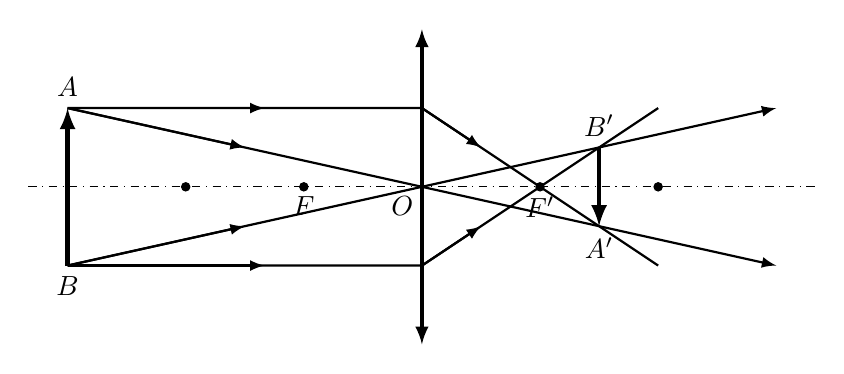
\begin{tikzpicture}[>=latex,scale=1]
  \draw[<->, very thick ] (0,2)--(0,-2);
  \draw[dashdotted](-5,0)--(5,0);
  \node at (-1.5,0)[below]{$F$};\node at (1.5,0)[below]{$F'$};\node at (-.25,-.25){$O$};
  \draw [fill=black] (-1.5,0) circle (1.5pt);
  \draw [fill=black] (1.5,0) circle (1.5pt);
  \draw [fill=black] (-3,0) circle (1.5pt);
  \draw [fill=black] (3,0) circle (1.5pt);
  %\draw [fill=black] (0,0) circle (1.5pt);
  \draw [->, ultra thick, >=latex] (-4.5,-1)node[below]{$B$}--(-4.5,1)node[above]{$A$};
  \draw [thick](-4.5,-1)--(0,-1)--(1.5,0)--(3,1);  \draw[thick] (-4.5,1)--(0,1)--(1.5,0)--(3,-1);
  \draw[->,thick, >=latex] (-4.5,-1)--(-2,-1);  \draw[->,thick, >=latex] (-4.5,1)--(-2,1);
  \draw[->, thick, >=latex] (-4.5,1)--(0,0)--(4.5,-1);
  \draw[->, thick, >=latex] (-4.5,-1)--(0,0)--(4.5,1);
  \draw [->, ultra thick, >=latex] (4.5/2,1/2)node[above]{$B'$}--(4.5/2,-1/2)node[below]{$A'$};
  \draw[->, thick, >=latex] (-4.5,1)--(-4.5/2,0.5);
  \draw[->, thick, >=latex] (-4.5,-1)--(-4.5/2,-0.5);
  \draw[->, thick, >=latex] (0,1)--(1.5/2,0.5);
  \draw[->, thick, >=latex] (0,-1)--(1.5/2,-0.5); 
\end{tikzpicture}
\end{document}